\documentclass{sigchi}

% Use this command to override the default ACM copyright statement (e.g. for preprints). 
% Consult the conference website for the camera-ready copyright statement.


%% EXAMPLE BEGIN -- HOW TO OVERRIDE THE DEFAULT COPYRIGHT STRIP -- (July 22, 2013 - Paul Baumann)
% \toappear{Permission to make digital or hard copies of all or part of this work for personal or classroom use is 	granted without fee provided that copies are not made or distributed for profit or commercial advantage and that copies bear this notice and the full citation on the first page. Copyrights for components of this work owned by others than ACM must be honored. Abstracting with credit is permitted. To copy otherwise, or republish, to post on servers or to redistribute to lists, requires prior specific permission and/or a fee. Request permissions from permissions@acm.org. \\
% {\emph{CHI'14}}, April 26--May 1, 2014, Toronto, Canada. \\
% Copyright \copyright~2014 ACM ISBN/14/04...\$15.00. \\
% DOI string from ACM form confirmation}
%% EXAMPLE END -- HOW TO OVERRIDE THE DEFAULT COPYRIGHT STRIP -- (July 22, 2013 - Paul Baumann)


% Arabic page numbers for submission. 
% Remove this line to eliminate page numbers for the camera ready copy
% \pagenumbering{arabic}


% Load basic packages
\usepackage{balance}  % to better equalize the last page
\usepackage{graphics} % for EPS, load graphicx instead
\usepackage{times}    % comment if you want LaTeX's default font
\usepackage{url}      % llt: nicely formatted URLs

% llt: Define a global style for URLs, rather that the default one
\makeatletter
\def\url@leostyle{%
  \@ifundefined{selectfont}{\def\UrlFont{\sf}}{\def\UrlFont{\small\bf\ttfamily}}}
\makeatother
\urlstyle{leo}


% To make various LaTeX processors do the right thing with page size.
\def\pprw{8.5in}
\def\pprh{11in}
\special{papersize=\pprw,\pprh}
\setlength{\paperwidth}{\pprw}
\setlength{\paperheight}{\pprh}
\setlength{\pdfpagewidth}{\pprw}
\setlength{\pdfpageheight}{\pprh}

% Make sure hyperref comes last of your loaded packages, 
% to give it a fighting chance of not being over-written, 
% since its job is to redefine many LaTeX commands.
\usepackage[pdftex]{hyperref}
\hypersetup{
pdftitle={Effects of In-Video Quizzes on Lecture Viewing Behavior in Coursera},
pdfauthor={LaTeX},
pdfkeywords={SIGCHI, proceedings, archival format},
bookmarksnumbered,
pdfstartview={FitH},
colorlinks,
citecolor=black,
filecolor=black,
linkcolor=black,
urlcolor=black,
breaklinks=true,
}

% create a shortcut to typeset table headings
\newcommand\tabhead[1]{\small\textbf{#1}}


% End of preamble. Here it comes the document.
\begin{document}

\title{Effects of In-Video Quizzes on Lecture Viewing in Coursera}

\numberofauthors{3}
\author{
  \alignauthor 1st Author Name\\
    \affaddr{Affiliation}\\
    \affaddr{Address}\\
    \email{e-mail address}\\
    \affaddr{Optional phone number}
  \alignauthor 2nd Author Name\\
    \affaddr{Affiliation}\\
    \affaddr{Address}\\
    \email{e-mail address}\\
    \affaddr{Optional phone number}    
  \alignauthor 3rd Author Name\\
    \affaddr{Affiliation}\\
    \affaddr{Address}\\
    \email{e-mail address}\\
    \affaddr{Optional phone number}
}

\maketitle

\begin{abstract}
In this paper we look at how users interact with quizzes embedded inside lecture videos (in-video quizzes) by analyzing video viewing logs on Coursera, a platform for hosting Massive Online Open Courses (MOOCs). We find that in-video quizzes are a common source and destination of video seeks. These seeks reflect behaviors such as searching for answers to the in-video quizzes within the video. There are spikes in view counts in the portions of the video surrounding in-video quizzes, as a result of reviewing and rewatching. We observe that some users follow quiz-oriented video navigation strategies, such as seeking directly from the start of the video to in-video quizzes, or between in-video quizzes. We discuss implications that these findings have on the design of online courses and MOOC platforms. % Other sources of seeks to in-video quizzes include the preceding section, where the learner may have found an answer. Potential design implications for video-viewing interfaces include making sure that users are easily able to refer to in-video quizzes. % suggest that video-viewing interface designs should make it easy for learners to refer to in-video quizzes. % Our findings that learners' rewatching and seeking activity peaks near in-video quizzes suggests that interfaces should enable learners to easily refer back to in-video quizzes.
\end{abstract}

\keywords{
	in-video quizzes; video analysis; log analysis; seeking; rewatching; Coursera; MOOC; online education \newline
}

\category{H.5.1.}{Information Interfaces and Presentation (e.g. HCI)}{Multimedia Information Systems: Video}

\begin{figure}
%\centering
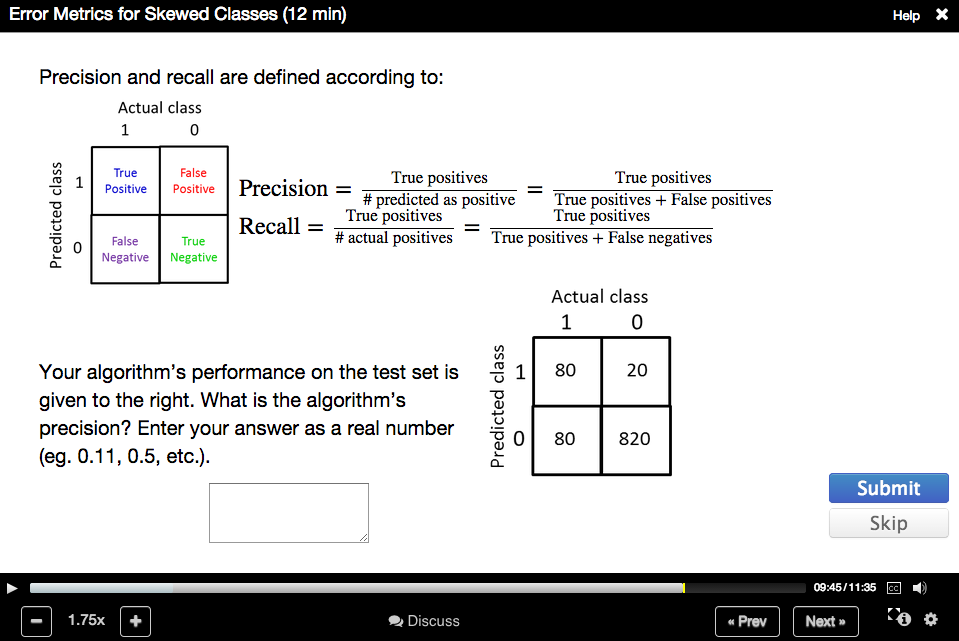
\includegraphics[width=1.0\columnwidth]{coursera}
\caption{An in-video quiz, from the ML4 course on Coursera. In-video quizzes are auto-graded questions embedded into a video and shown at a certain timestamp. They can be either multiple choice, multiple selection, or numeric free-response. Their locations are indicated on the progressbar by a yellow tick.}
\label{fig:coursera}
\end{figure}

\section{Introduction}

In-video quizzes, which are commonly featured in courses on platforms such as Coursera, are questions that users are asked to answer upon reaching a certain point in the video, as shown in Figure~\ref{fig:coursera}. In-video quizzes are auto-graded; the majority we observe in the Machine Learning course and other courses on Coursera are either multiple-choice or multiple-selection, though there also exist a few numeric-response quizzes.

In-video quizzes differ from standard quizzes in that users do not leave the video viewer interface when they encounter a quiz, so users can easily seek elsewhere upon encountering the quiz -- seeking backward to find answers to the quiz, seeking forward to skip the quiz, etc.
The presence of in-video quizzes inside videos can thus influence users' video viewing behaviors,
relative to the default linear video-viewing model.

In this paper, we analyze video-viewing logs of the Machine Learning course, iteration 4 on Coursera. We identify and discuss a set of video viewing behaviors associated with in-video quizzes that we observe in these logs, specifically:

\begin{itemize}
\item The region preceding in-video quizzes are a common destination for video seeks.
\item In-video quizzes are a common sources of video seeks.
\item Users often seek backward from in-video quizzes to find the answer to the in-video quiz.
\item Some users appear to be following a strategy of seeking directly to the in-video quizzes
\item Some users tend to jump from one in-video quiz to the next, skipping the video segments
\item Users do not tend to skip over in-video quizzes
\end{itemize}

These behaviors suggest that certain viewers attach high importance to in-video quizzes and frequently refer to them, and suggests that video-viewing interfaces should perhaps make it easier for users to refer to the in-video quiz associated with the segment they are viewing.

\newpage

\section{Related Work}

Kim et al perform an analysis of reasons for peaks in viewing and seeking while viewing lectures \cite{juho}. They find that users steadily leave videos over time, a phenomenon they refer to as \emph{video dropout}, and that visual transitions, such as slide transitions, tend to result in \emph{interaction peaks}, such as users seeking back to the previous slide. They also present a video viewer that encourages video navigation to interaction peaks  \cite{juho2}. However, the courses that they perform their video log analysis on do not have in-video quizzes, hence they are unable to report on viewing peaks and seeking behaviors that result from in-video quizzes. We similarly found in our own analysis that there are many peaks in seeking behavior that can be accounted for by slide transitions, however in-video quizzes tend to also be a major factor in causing peaks in video seeking.

Guo et al discuss the effects of video properties on such as video length on viewer engagement \cite{guovideo}. They find that users become less engaged as videos grow longer, which is related to the problem of in-video dropout. However, they do not analyze the effects on in-video quizzes on viewer engagement, because the courses they analyze do not have in-video quizzes. In this paper, we argue that in-video quizzes encourage viewer engagement, as indicated by the increase in rewatching and seeking behavior in the regions of the video surrounding the in-video quiz.

Guo et al discuss factors that contribute to nonlinear navigation through MOOCs \cite{guodemographics}. They discuss examples of nonlinear navigation such as jumping back to previous lectures, rewatching videos, and going back from asssements to refer to lectures. Our present work is focused on navigation within videos as opposed to within MOOCs. However, we find that in-video quizzes, being a form of assessment that is embedded into the videos, trigger similar backjumps and reviews within a video that Guo et al discuss at the course-level in their paper.

Andersson et al find that learners differ in the ways they engage with online courses: some only watch videos (``viewers''), some only do assignments (``solvers''), and some do both (``all-rounders'') \cite{ashton}. The courses they analyzed were previous offerings of the Machine Learning course on Coursera that is the focus of this work, and we have found that their findings still apply in the fourth iteration of the course. These differences between learners' engagement patterns are relevant to our work analyzing in-video quizzes, as they help explain why we find that some users' viewing behaviors seem to be aimed towards solving in-video quizzes rather than watching videos.

In-video quizzes are not new; there are many past systems that embed quizzes into multimedia \cite{multimedia}, and they are believed to have positive effects on learning \cite{embedded}. However, to our knowledge, our paper is the first analysis of the effects on in-video quizzes on learners' rewatching and seeking behavior in the context of MOOCs.

\newpage

\section{Materials}

The course we are analyzing in this work is the fourth iteration of the Machine Learning course on Coursera, which we will abbreviate as \textit{ML4}. There are 113 lecture videos in the course, totaling 19.5 hours of video content, with an average length of 10 minutes per video.  With 108 in-video quizzes over 19.5 hours of video, this averages out to one in-video quiz for every 11 minutes of video.

Of the 113 videos, 93 videos (82\%) have 1 in-video quiz, 13 videos (12\%) have no in-video quizzes, 6 videos (5\%) have 2 in-video quizzes, and 1 video (1\%) has 3 in-video quizzes. Videos with no in-video quizzes tend to be optional lectures covering interesting applications of machine learning, or are introductory videos that explain what will be covered next in the course. In videos with 1 in-video quiz, the in-video quiz tends to be placed at the end of the video and is followed by only a summary and no new content. In videos with multiple in-video quizzes, they tend to be evenly spaced out through the video. Although 60 thousand users began watching the first lecture, the number of viewers drops down to 13 thousand by the half-point of the course, agreeing with the gradual dropout from courses that previous studies have observed \cite{dropout}.

We use viewing logs observed on lectures from ML4 to illustrate certain phenomenon we found to hold true across a wide sample of videos in ML4. One of the lectures we use in our examples is Lecture 68: Error Metrics for Skewed Classes, a 12-minute video containing a single in-video quiz which asks for a free-response numeric answer. Another is Lecture 13: Matrices and vectors, a 9-minute video containing two in-video quizzes, of which the first is multiple-selection (4 checkboxes), and the second is multiple-choice (4 radioboxes).

\section{Methodology}

The Coursera logs we used for our analysis come with an action (such as play, pause, or seek) associated with a point in the video, and a timestamp. We use these logs to reconstruct the portions of the video that the user has seen, with a technique similar to the one described in \cite{juho} -- if we observe a play event associated with video position p, followed by another event at video position p+i, we can assume that the user watched that segment of the video.

The seek events in the logs specify only the destination of the seek and the timestamp at which it occurred, but not the origin (the logs tell us where in the video the user seeked to, but not where the user seeked from). However, we were likewise able to reconstruct the seek time origins based on the previous event -- for example, if the user started playing from video position p at timestamp t, and we observe a seek event at timestamp t+i, then we assume the seek originated from video position p+i (or p+i*2 if the user is playing back the video at 2x speed, etc).

Additionally, we observed that many seek events tend to occur in rapid succession as the user narrows down on the actual target. For example, if the user is seeking via the keyboard, if they are at the beginning of the video and their seek target is 3 minutes into the video, they will press the right-arrow repeatedly until they reach the destination, resulting in a large number of small, noisy seek events, rather than the user's intended seek from 0 to 3 minutes that we are interested in analyzing. Because we are primarily interested in where the user ends up seeking to, rather than the individual seek operations that got them to that point, if there are seek events that occur within 10 seconds of one each, we group them together into a single unit which we will call a \textit{seek chain}. When we analyze seeking in this paper, as well as seek sources and destinations, we will be analyzing seek chains rather than raw seek events, to reduce noise from repeated seeks.

Some play and pause events are automatically generated when the user reaches certain points in the video. For example, when a user clicks on a video in the lecture list, it will auto-play, and a play event is automatically logged at video time 0. When the user reaches an in-video quiz or the end of the video, a pause event is automatically logged at that point. When the user clicks ``continue'' after answering an in-video quiz, the video automatically continues playing, and a play event is logged.

A limitation of this dataset is that if the user closes their browser window or their network disconnects, this event does not show up in the log, and hence there is ambiguity as to what they watched. For example, if a user starts playing a video at time t, and this play event is the last logged event, we know that the user must have closed their browser prior to the next in-video quiz or the end of the video (otherwise a pause event would have been automatically logged), however we do not know exactly when . We address this ambiguity by treating it as though the user had immediately stopped watching after that last play event, so we do not include the last (unknown) segment that users who quit before the end have watched in the video.

We observed inconsistencies in the view logs for some users (roughly 1\%) -- for example, observing seek and pause events from the user before we observe any play events -- so we excluded those users from our analysis.

\begin{figure}
%\centering
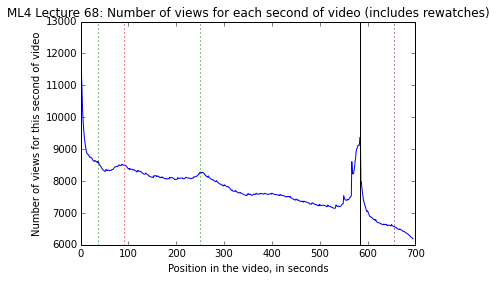
\includegraphics[width=1.0\columnwidth]{videoviewsall}
\caption{Number of times each second of video was viewed. Black lines indicate in-video quizzes, green lines indicate slide boundaries, the red line indicates a portion where some code was shown, the purple line indicates the start of the end-of-video summary -- portion where the slides are hidden and only a talking head is shown. We can observe a steady decrease in the number of views with increasing time (in-video dropouts), with some bumps due to slide transitions. However, there is an increase in the number of views in the portion immediately preceding the in-video quiz, where the answer can be found.}
\label{fig:videoviewsall}
\end{figure}

\begin{figure}
%\centering
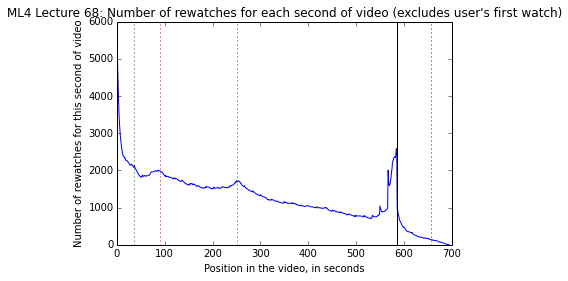
\includegraphics[width=1.0\columnwidth]{rewatches}
\caption{Number of times each second of video was viewed, excluding each user's first view. There is an increase in the number of rewatches in the portion immediately preceding the in-video quiz (black line), where the answer can be found.}
\label{fig:rewatches}
\end{figure}

\begin{figure}
%\centering
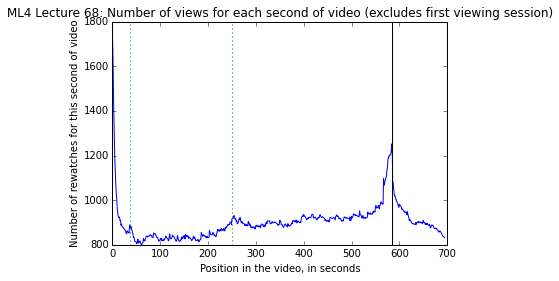
\includegraphics[width=1.0\columnwidth]{rewatchingsessions}
\caption{Number of times each second of video was viewed in rewatching sessions. This excludes logs from within an hour of the user first watching the video. During rewatching sessions, users will often go straight to the region surrounding the in-video quiz (black line), and skip over the rest of the video.}
\label{fig:rewatchingsessions}
\end{figure}

\begin{figure}
%\centering
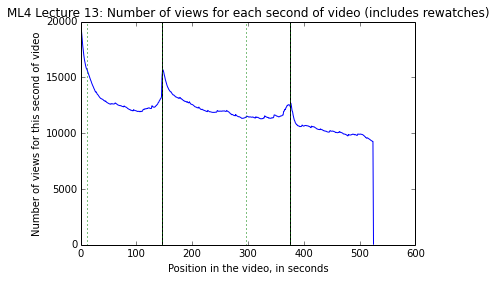
\includegraphics[width=1.0\columnwidth]{watched13}
\caption{Number of times each second of video was viewed. Black lines indicate in-video quizzes, green lines indicate slide boundaries. Even if there are multiple in-video quizzes, an increase in rewatching is observed around each of them.}
\label{fig:watched13}
\end{figure}

\begin{figure}
%\centering
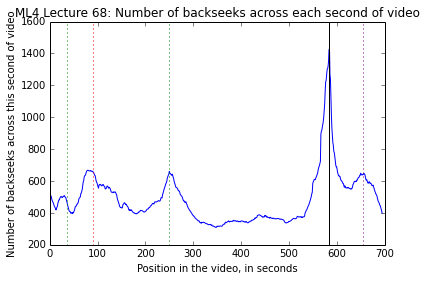
\includegraphics[width=1.0\columnwidth]{backseeks}
\caption{Number of times a backwards seek chain crossed a given second of video. Peaks occur on slide boundaries (green lines), indicating users are going back to the previous slide. Small peaks also occur where code is shown (red line) and at the start of the end-of-video summary (purple line). Peaks also occur both before and after the in-video quiz (black line). Peaks before in-video quizzes are likely users seeking answers to the questions. Peaks after in-video quizzes are likely users who wish to review the content covered by the in-video quiz.}
\label{fig:backseeks}
\end{figure}

\begin{figure}
%\centering
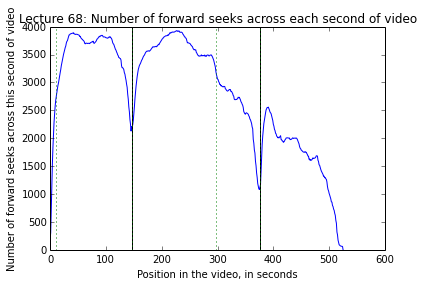
\includegraphics[width=1.0\columnwidth]{fwdseek13}
\caption{Number of times a forwards seek chain crossed a given second of video. Green lines indicate slide boundaries, black lines indicate in-video quizzes. Dips occur at in-video quizzes, indicating that users are not attempting to skip over the in-video quizzes.}
\label{fig:fwdseek13}
\end{figure}

\section{In-Video Quiz Answering Rates}

TODO: Statistics on:

\begin{enumerate}
\item What percent of users who start watching the video reach the in-video quiz? (ie, play a point in the video that is at or past the in-video quiz)
\item What percent of users who reach the in-video quiz attempt it? What percent skip over it (play a point in the video that is past the in-video quiz, but is not at the quiz)? What percent press the play/skip button (reach the in-video quiz, but continue playing without having submitted an answer)?
\item What percent of users who attempt in-video quizzes eventually answer them correctly? What is the mean number of tries before a correct answer? What percent of users navigate away from the in-video quiz before answering it correctly? How many navigations away on average?
\end{enumerate}

\section{Increased rewatching near in-video quizzes}

We hypothesized that if encountering in-video quizzes is causing users to try to find answers to the quiz question in the video, this should be reflected in the viewing logs. Namely, we would expect to see increased re-watching of the portion prior to the in-video quiz where the answer is located, as well as seeks that originate from the in-video quiz and go backwards to where the answer was located. We show examples of these phenomenon in this section.

We see in Figure~\ref{fig:videoviewsall} that the portion of the video preceding the in-video quiz tends to receive more views. We also observe in that figure a trend of less views for portions of the video that occur later, which can be explained as in-video dropout, which occurs as a consequence of users tending to watch videos linearly \cite{juho}.

To measure how much more, we did a linear regression on the videos

We believe the increase in number of views surrounding the in-video quiz is due to the user rewatching the portion preceding the in-video quiz, perhaps hoping to find an answer to the quiz. Indeed, if we exclude each user's first-time watch, and look only at what users are rewatching in aggregate, we still observe this peak in number of rewatches around the first in-video quiz, as shown in Figure~\ref{fig:rewatches}. This effect is further amplified if we observe users' behaviors in a seperate rewatching session that occurs at least 1 hour after they initially open the. We find that in these rewatching sessions, many will just seek directly to the in-video quiz, as indicated in Figure~\ref{fig:rewatchingsessions}.

An alternative explanation for the increase in the number of rewatches surrounding the in-video quiz could be that in videos with a single in-video quiz (the most common format in ML4), the in-video quiz occurs towards the end of the video. The portion immediately preceding the in-video quiz also tends to be a fully-built out slide, that summarizes the content of the video. Hence, it could simply be the case that users are rewatching that particular segment, because the video content is a good summary of the entire video, rather than having anything to do with the presence of the in-video quiz. However, if we look at videos with multiple in-video quizzes, we still observe the peak of rewatching around the in-video quizzes as shown in Figure~\ref{fig:watched13}, hence the rewatching is not due to just the position of the in-video quiz at the end of the video.

We also observe a peak in the number of backwards seek chains that cross regions surrounding the in-video quiz, as shown in Figure~\ref{fig:backseeks}. Backwards seek chains originating from the in-video quiz itself can be attributed to user behavior where the user is seeking backwards to find an answer to the in-video quiz. Backwards seek chains originating from past the in-video quiz can be attributed to users wishing to review the content tested in the in-video quiz.

Because Coursera does not enforce that users take in-video quizzes, we wondered whether users are explicitly skipping across the in-video quizzes to avoid taking them. As illustrated in Figure~\ref{fig:fwdseek13}, we found that this does not tend to be the case. On the contrary, there is actually a dip in the number of forward seeks that cross over the in-video quiz, so users are explicitly trying not to skip the in-video quizzes. This low number of forward seeks crossing over the last in-video quiz in this example might be attributed to the fact that it is at towards the end of the video, so the user may know that there is no new content to find towards the end. However, if we look at the first in-video quiz in the example, we also observe a dip in the number of forward-seeks over the in-video quiz, even though there is important content in the video after it.

Our findings in this section suggest that users tend to attribute importance to in-video quizzes, because they rewatch the regions surrounding them, tend to backseek to review the materials preceding the quiz, and do not forward-seek over quizzes to avoid taking them.

\section{Causes of seeks to and from In-Video Quizzes}

\begin{figure}
%\centering
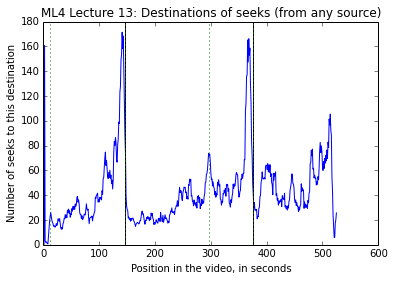
\includegraphics[width=1.0\columnwidth]{seekdestinations}
\caption{Destinations of seek chains in a video, regardless of source. Black lines indicate in-video quizzes, green lines indicate slide transitions. We can see that the most common places people seek to are to the very beginning of the video, as well as right before the in-video quiz (this includes both users wishing to review the part in front of the in-video quiz, as well as users who wish to take the in-video quiz, as Coursera's interface does not allow users to jump directly to an in-video quiz). There is also a smaller peak near the slide transition.}
\label{fig:seekdestinations}
\end{figure}

\begin{figure}
%\centering
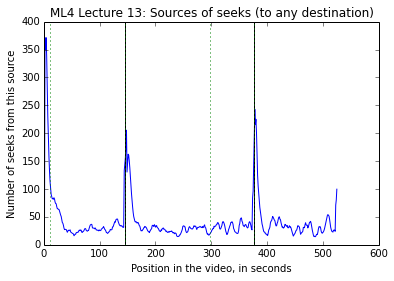
\includegraphics[width=1.0\columnwidth]{seeksources}
\caption{Sources of seek chains in a video, regardless of destination. Black lines indicate in-video quizzes, green lines indicate slide transitions. We can see that the most common places people seek from are the beginning of the video, as well in-video quizzes.}
\label{fig:seeksources}
\end{figure}

\begin{figure}
%\centering
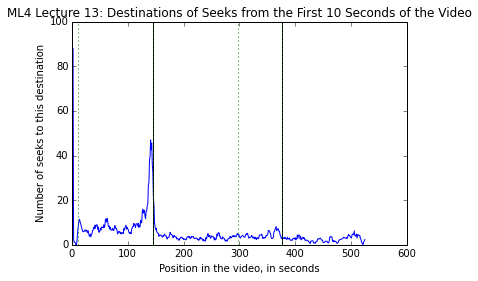
\includegraphics[width=1.0\columnwidth]{seekdest0}
\caption{Destinations of seeks that originate from the first 10 seconds within the video. Black lines indicate in-video quizzes, green lines indicate slide boundaries. We can see that apart from seeks that return to the start of the video, the most common seek destination is the portion preceding the first in-video quiz.}
\label{fig:seekdest0}
\end{figure}

\begin{figure}
%\centering
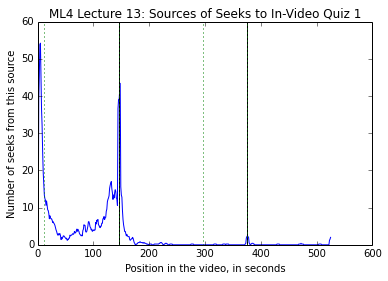
\includegraphics[width=1.0\columnwidth]{seeksrc1}
\caption{Sources of seeks that end up in the 10 seconds preceding the in-video quiz. Black lines indicate in-video quizzes, green line indicate slide boundaries. We see that the most common seek source is the start of the video. There are also backward-seeks from the portion immediately after the in-video quiz, which can be users wishing to review the material tested in the in-video quiz, as well as forward-seeks from the portion immediately preceding the in-video quiz, which can be users who have found the answer and wish to answer the in-video quiz.}
\label{fig:seeksrc1}
\end{figure}

\begin{figure}
%\centering
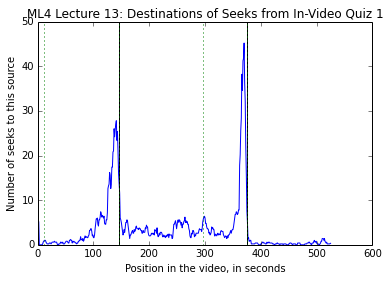
\includegraphics[width=1.0\columnwidth]{seekdest1}
\caption{Destinations of seeks that originate from the 10 seconds following the first in-video quiz. Black lines indicate in-video quizzes, green lines indicate slide boundaries. We can see that the most common seek destination is the portion preceding the second in-video quiz. There are also users who seek to the section before the in-video quiz, presumably looking for the answer to the quiz.}
\label{fig:seekdest1}
\end{figure}

\begin{figure}
%\centering
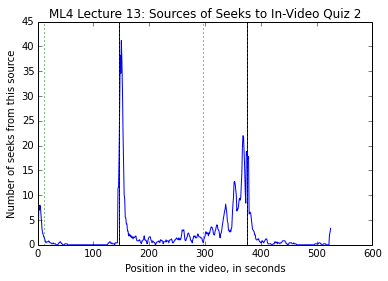
\includegraphics[width=1.0\columnwidth]{seeksrc2}
\caption{Sources of seeks that end up in the 10 seconds preceding the second in-video quiz. Black lines indicate in-video quizzes, green line indicate slide boundaries. We see that the most common seek source is the first in-video quiz. There are also backward-seeks from the portion immediately after the in-video quiz, which can be users wishing to review the material tested in the in-video quiz, as well as forward-seeks from the portion immediately preceding the in-video quiz, which can be users who have found the answer and wish to answer the in-video quiz.}
\label{fig:seeksrc2}
\end{figure}

\begin{figure}
%\centering
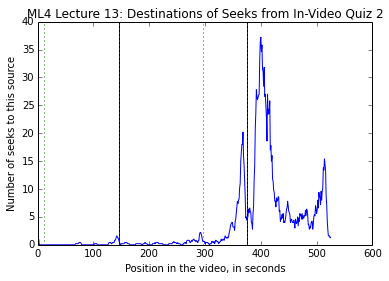
\includegraphics[width=1.0\columnwidth]{seekdest2}
\caption{Destinations of seeks that originate from the 10 seconds following the second in-video quiz. Black lines indicate in-video quizzes, green lines indicate slide boundaries. We see that users seek towards the end section, where the video is summarized.}
\label{fig:seekdest2}
\end{figure}

We observe that the portion of the videos directly preceding in-video quizzes tend to be the most common destination of video seek chains, as indicated in Figure~\ref{fig:seekdestinations}. Bin-summarize smoothing is used to increase the salience of patterns in that figure, as well as subsequent figures \cite{smoothing}. This is perhaps expected, because they are saliently marked on the video progressbar, and are the most interactive portion of the video. Users may be seeking to before in-video quizzes either because they are seeking an answer to the in-video quiz, or because they want to look at the in-video quiz -- because Coursera's interface does not allow users to seek directly to in-video quizzes, both intents will appear in logs as seeks to directly before the in-video quiz.

We additionally observed that, apart from the very beginning of videos, in-video quizzes also tend to be a common source of video seek chains, as indicated in Figure~\ref{fig:seeksources}. Users might be seeking directly backward, to help them answer the in-video quiz, which agrees with the peak in back-seeking over in-video quizzes we observed in the previous section. Alternatively, users might be seeking forwards, perhaps seeking from the first in-video quiz to the next one, and from the second in-video quiz to the video summary at the end.

Based on these observations that in-video quizzes are common seek sources and destinations, we wondered whether any users were following a strategy of seeking to the quizzes first, before looking at the preceding video. We will analyze this below by seeing where the sources and destinations of seeks to/from in-video quizzes are.

% We wondered whether any users were following a strategy of seeking to the quizzes first, before looking at the preceding video. Such activity would show up in seek logs as seeks from the beginning of the video to right before the first in-video quiz (Coursera's interface does not allow users to seek directly to an in-video quiz, hence a user attempting to see the in-video quiz would end up seeking to a few seconds before the in-video quiz).

Figure~\ref{fig:seekdest0} illustrates the destinations of seek chains originating from the first 10 seconds of the video: as we can see, the most common seek target is the first in-video quiz. Figure~\ref{fig:seeksrc1} illustrates the sources of seek chains that end up at the in-video quiz: as we can see, the most common seek source is the start of the video, although there are users who backseek from the following section as well.

This behavior of jumping to the next in-video quiz holds true for the following in-video quizzes as well. Figure~\ref{fig:seekdest1} shows that the most common seek destination starting from the first in-video quiz is the second in-video quiz. Figure~\ref{fig:seeksrc2} likewise shows that the most common source of seeks to the second in-video quiz is from the first in-video quiz. Finally, if we observe seeks from after the last in-video quiz, we find that users tend to go to the end section of the video, where the video is summarized, as shown in Figure~\ref{fig:seekdest2}.

Hence, we have found that in-video quizzes are major sources and destinations of seek chains. Based on the sources and destinations of seek chains going to/from in-video quizzes, the seeking behaviors that we observe around in-video quizzes include:

\begin{itemize}
\item Users seeking from one quiz to the next, presumably aiming to answer the in-video quiz questions
\item Users seeking backwards to the quiz from the immediately following section, to review its contents
\item Users seeking forward to the in-video quiz, presumably to respond to the question after having found the answer, or to remind themselves of what the quiz was asking them to find.
\end{itemize}

\section{Discussion}

The peaks in rewatching and seeking behaviors that we observed around in-video quizzes suggest a number of possible interface improvements that could be experimented with. Coursera currently does not allow users to easily skip directly to in-video quizzes, instead requiring them to go to the preceding few seconds of videos. As indicated by how we observed that in-video quizzes were one of the most common destinations for seek chains, skipping to in-video quizzes should  be made easier, perhaps via improved scrubbing techniques. We also observed that users tend to revisit in-video quizzes during rewatching sessions. This suggests that it may be beneficial if users had an easy way to refer back to the in-video quizzes they had previously encountered while reviewing.

A limitation in this study is that it is impossible to determine exactly what point users who simply closed their browser windows stopped watching videos at. This is due to the Coursera's lack of a second-by-second heartbeat showing whether the user is still connected -- we can observe the last event from the user (perhaps a play event), but we do not know how much time elapsed between that event and the user closing their browser, so we do not know precisely where the final segment watched by the user ended. EdX does not currently implement a heartbeat for determining user disconnections either, so this is a limitation shared by other studies relying on EdX data. To better be able to study users' interactions with videos, and to understand exactly where users lose engagement with videos and close them, these platforms need to be able to determine when users close their browsers.

Because our study did not perform any A/B tests varying the number of in-video quizzes, we do not know whether in-video quizzes have any effect on the overall video watching completion rate, or their effects on in-video dropout rates. Due to the fact that few users attempt to skip in-video quizzes by forward-seeking over them, and that the in-video dropout rate in the portion directly preceding the in-video quiz appears to decrease rather than increase, we speculate that the presence of in-video quizzes may be beneficial for keeping users engaged and to continuing to watch the video.

\section{Conclusion}

We have presented ways that in-video quizzes influence users' video watching behaviors, as indicated by seeking logs on various videos in the ML4 course on Coursera. We find that users' seeking and rewatching behaviors in videos are influenced by the presence of in-video quizzes. Specifically:

\begin{itemize}
\item There are peaks in rewatching behavior in the regions surrounding the in-video quiz. In particular, we see a large amount of back-seeking from in-video quizzes to the immediately preceding video section. This is likely due to users seeking answers to in-video quizzes.
\item Many users skip directly to the in-video quizzes during rewatching sessions. Hence, they may be using these as a way to test themselves, to determine whether or not they need to review that video. 
\item Users do not tend to seek forwards over in-video quizzes to skip over them.
\item In-video quizzes are a common source of seek chains within videos. Users tend to seek backward to find answers, or forward to the next in-video quiz.
\item In-video quizzes are a common destination of seek chains within videos. Users tend to seek from the preceding video segment where the answer can be found, from the beginning of the video, or from the preceding in-video quiz.
\end{itemize}

\bibliographystyle{acm-sigchi}
\bibliography{invideo}
\end{document}
